% ════════════════════════════════════════════
% 2. 分析思路
% ════════════════════════════════════════════
\section{分析思路}

\subsection{分析框架}

分析按“数据诊断—数据整理—回归建模—效应测算”四个环节递进，前一环节的输出是后一环节的输入，四环节共用同一份只读原始数据与同一套变量口径。图\ref{fig:route}给出四个任务的分工：任务 1 判断数据能支持什么样的模型，任务 2 把原始表整理为分析数据，任务 3 估计并诊断回归模型，任务 4 把系数还原为曝光次数与倍数。

\begin{figure}[htbp]
  \centering
  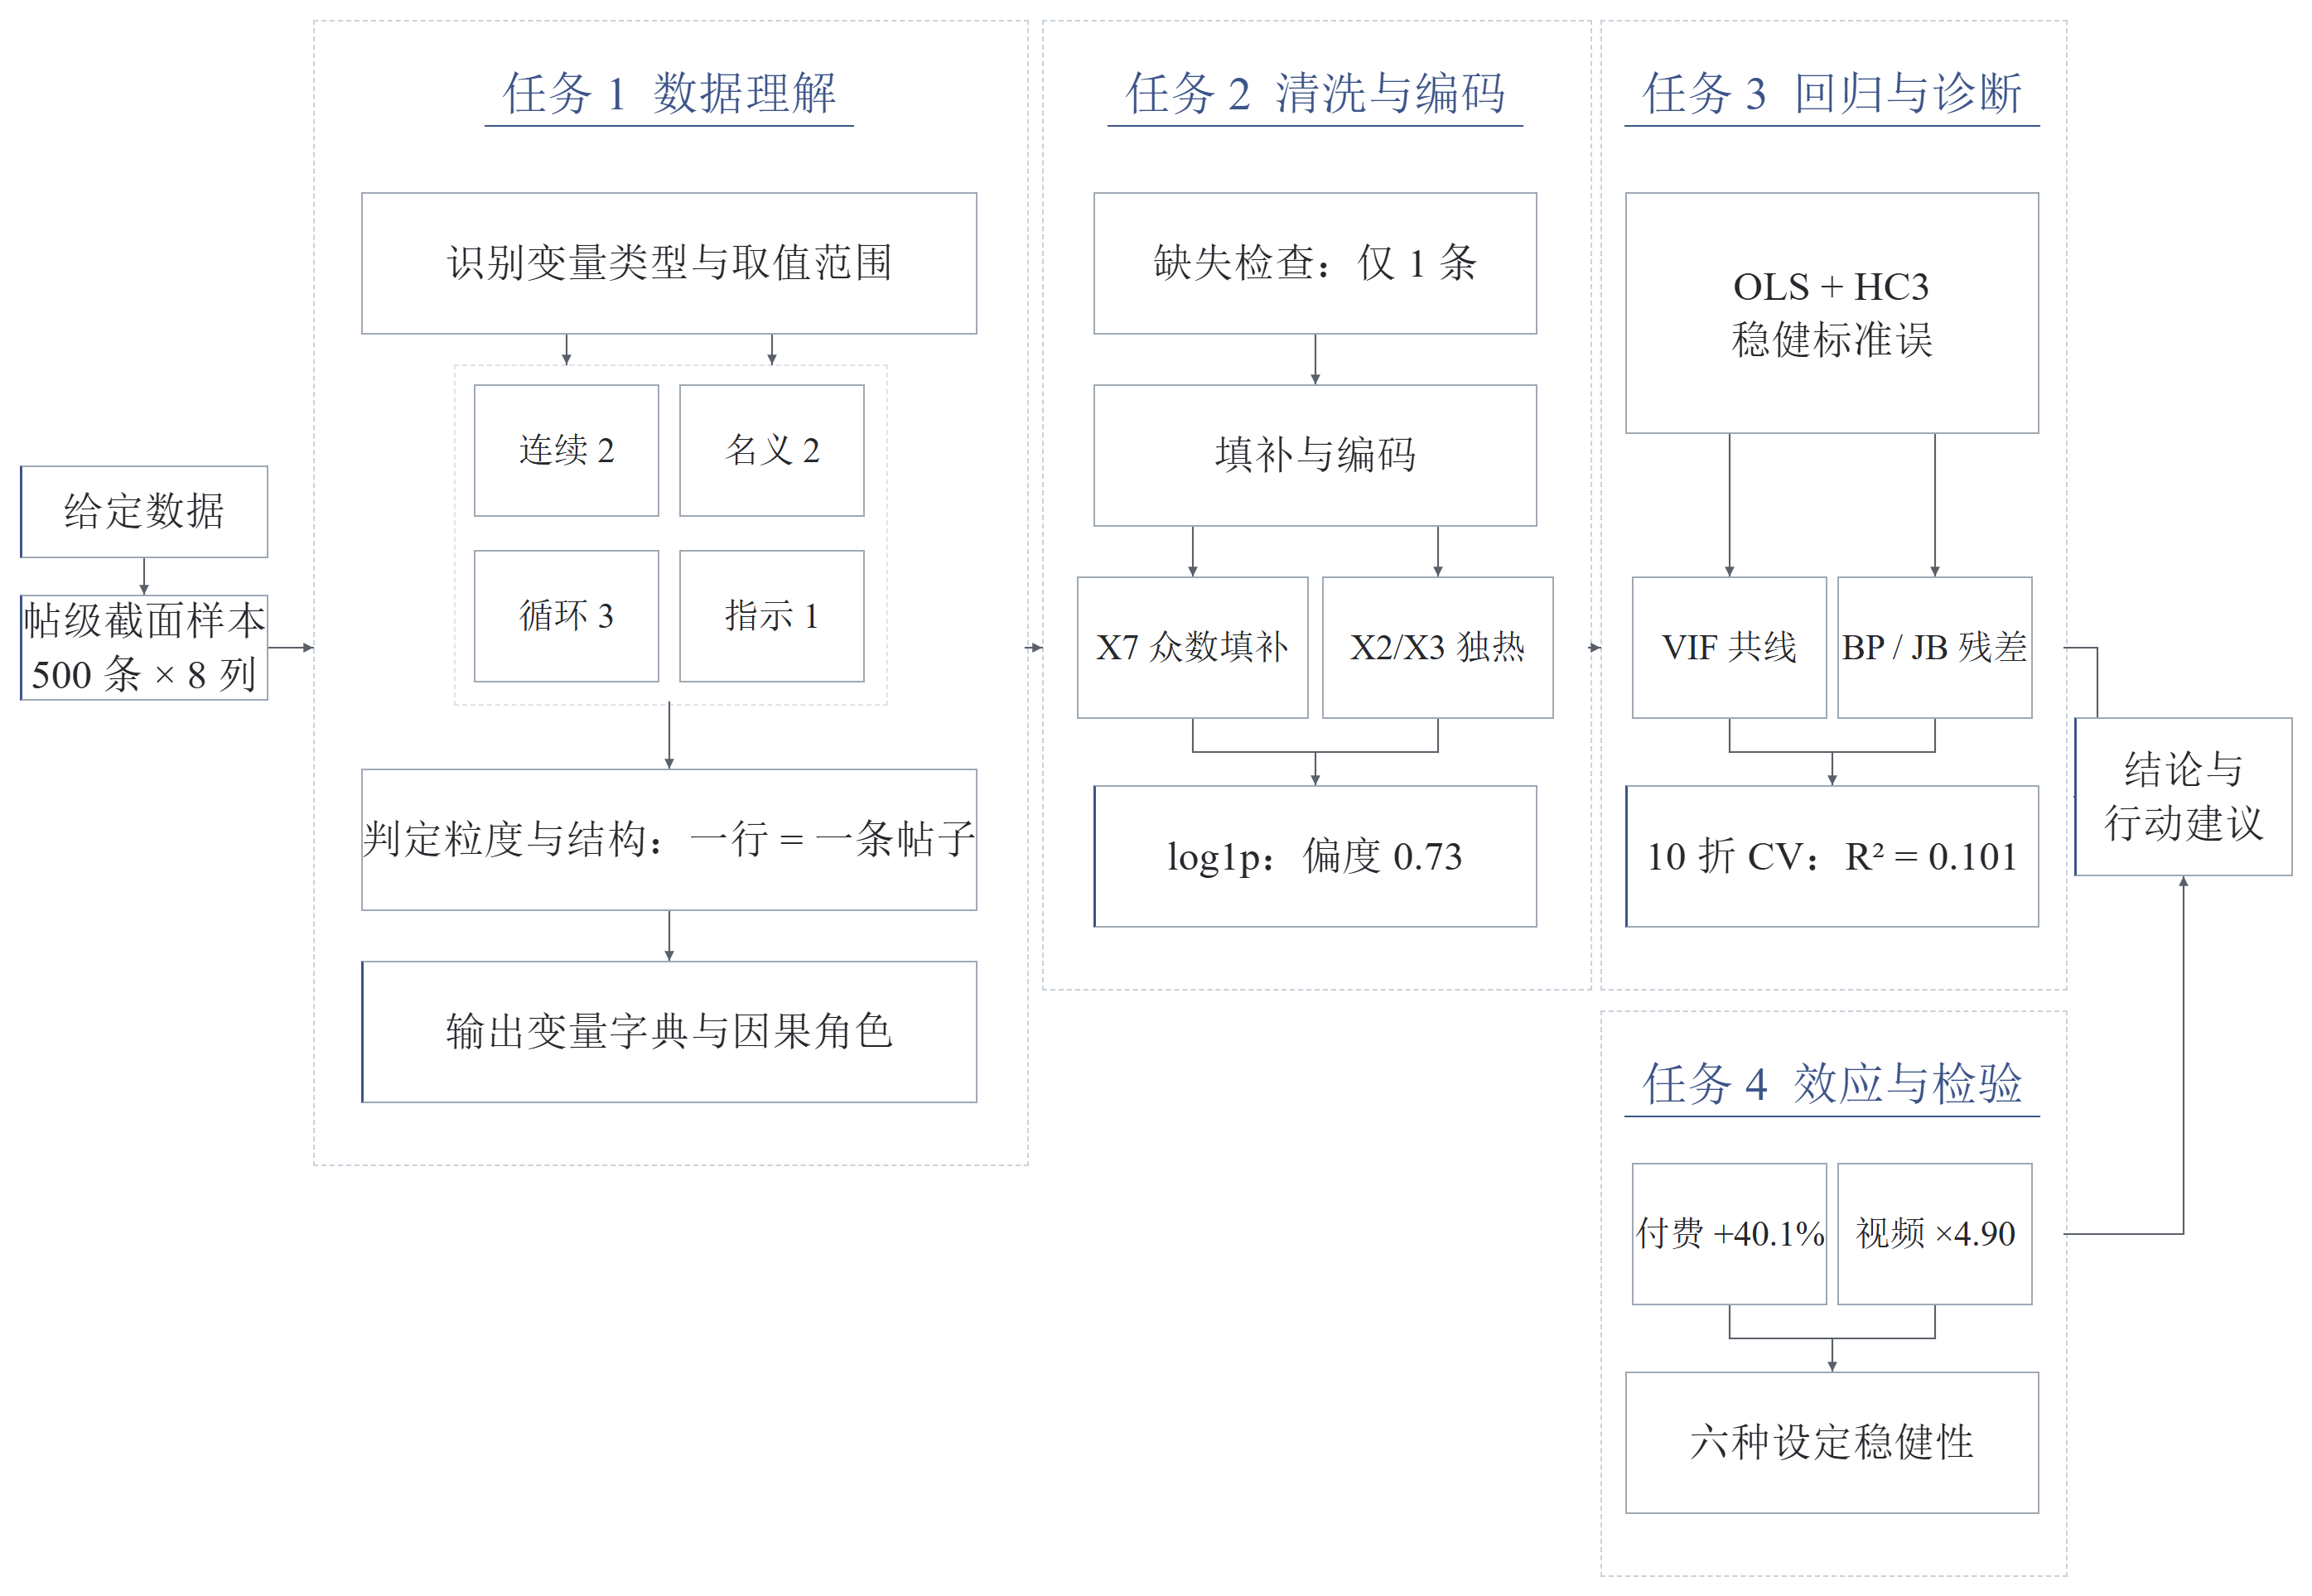
\includegraphics[width=0.84\textwidth]{../求解/临时产物/图0_技术路线.png}
  \caption{分析框架：四个任务的数据流与关键判据}
  \label{fig:route}
\end{figure}

\subsection{关键判据}

各环节的取舍都由可复核的阈值决定，避免凭经验选择。共线判别使用三项判据：变量间相关系数绝对值不低于 0.9、以其中一个变量对另一个做辅助回归的解释度不低于 0.9、月内方差占比低于 5\%；三项同时满足即视为同一变异维度，只能保留其一。变换判据看偏度与峰度是否落入 $[-1,1]$ 量级，$\log(1+Y_1)$ 变换后偏度 0.73、峰度 0.82，据此确定因变量尺度。模型选择不看样本内拟合，而看十折交叉验证的 $R^2$ 与 RMSE；推断口径看残差检验，Breusch--Pagan 与 Jarque--Bera 均拒绝同方差与正态假设，因此统一采用 HC3 稳健标准误。

\subsection{章节安排}

第 3 章对应题面 2.1，给出数据结构、变量类型与分布；第 4 章对应 2.2 与 2.3，说明缺失处理、编码变换与共线判定；第 5 章给出样本结构与变量关系的描述性分析；第 6 章对应 2.4 的前半部分，完成建模、诊断、预测能力评估与方差分解；第 6.6--6.7 节对应 2.4 的效应解释部分，给出付费、类型、主题的效应测算与稳健性检验；第 7 章集中呈现图形证据，第 8 章汇总结论与适用边界。
